%%%%%%%%%%%%%%
%       Curriculum Vitae     %
% 	    Bojan Popržen      %
%%%%%%%%%%%%%%

\documentclass[11pt]{article}


%%%%%%%
% Packages %
%%%%%%%

\usepackage[margin=15mm]{geometry}
\usepackage{tikz}
\usepackage{graphicx}
\usepackage{epstopdf}
\usepackage{hyperref}
\usepackage{array}
\usepackage{paralist}
\usepackage{ifthen}
\usepackage{longtable}


\usetikzlibrary{arrows,decorations,positioning}

%%%%%%%%
% Page setup %
%%%%%%%%

% Remove implicit indentations and separations
\setlength{\parindent}{0pt}
\setlength{\itemsep}{0pt}


% Defining the layout of tabular columns (0.96)
\newcolumntype{L}{>{\raggedleft}p{0.17\textwidth}}
\newcolumntype{D}{p{0.79\textwidth}}

\newcolumntype{A}{>{\raggedleft}p{0.08\textwidth}}
\newcolumntype{B}{p{0.88\textwidth}}

%%%%%%%%%%
% colors %
%%%%%%%%%%

\definecolor{maincolour}{HTML}{191970}

%%%%%%%%%%%%%%%%%%%%%%%%%%%%%%
% Custom command definitions %
%%%%%%%%%%%%%%%%%%%%%%%%%%%%%%

% Custom rules: thick horizontal, thin horizontal, vertical
\newcommand{\HRule}{\rule{\linewidth}{0.5mm}}
\newcommand{\SRule}{\rule{\linewidth}{0.2pt}}
\newcommand{\VRule}{\color{lightgray}\vrule width 0.5pt}

% "Divider" that comes after each sub-heading
\newcommand{\divider}{\vskip-7pt\HRule\hfill\vskip-1.1em\SRule\vskip1em}

% This is the command used to produce each sub-heading.
% Usage: \heading{Heading text}.
\newcommand{\heading}[1]{
	{\LARGE \bf \textcolor{maincolour}{#1}}
	\textcolor{maincolour}{\divider}
}

% Command used to make an education-related entry
% Usage: \educationentry{Optional arg - Vertical space after}{Diploma}{Faculty}{University}{Details}
\newcommand{\educationentry}[5][0.25em]{
	\begin{tabular}{@{}l} % supress the space
		{\bfseries #3}	% Faculty
	\end{tabular}
	\hfill
	\begin{tabular}{l@{}}
		{\bfseries #4} % University
	\end{tabular} 
	\newline
	\begin{tabular}{@{}l}
		{#2}
	\end{tabular}
	\vspace{0.5em}
	% \hfill
	#5
}

% Command used to make an project-related entry
% Usage: \educationentry{Optional arg - Vertical space after}{Technologies}{Project name}{Web-site}{Details}
\newcommand{\projectentry}[5][0.25em]{
	\begin{tabular}{@{}l} % supress the space
		{\bfseries #3}	% Project name
	\end{tabular}
	\vspace{0.3em}
	\hfill
	\begin{tabular}{l@{}}
		{#4} % Web-site
	\end{tabular} 
	\newline
	\begin{tabular}{@{}l}
		{#2} % Technologies
	\end{tabular}

	\vspace{0.25em}
	#5
}

%% Command used to make the |Timeline|educationentry| table 
%% Usage: \timelinetable{firstrowfirstcol & firstrowsecondcol \\ secondrowfirstcol & secondrowsecondcol}
\newcommand{\timelinetable}[1]{
	\begin{tabular}{L!{\VRule}D}
		#1
	\end{tabular}
	\\[0.5em]
}

\newcommand{\timelinetableprojects}[1]{
	\begin{longtable}{A!{\VRule}B}
		#1
	\end{longtable}
	% \\[0.5em]
}


%%%%%%%%%%%%%
% START OF DOCUMENT %
%%%%%%%%%%%%%

\begin{document}

% Avoid printing page numbers
\pagestyle{empty}

%%%%%%%%%%%
% MAJOR HEADING %
%%%%%%%%%%%

\begin{tikzpicture}[remember picture, overlay, transform shape]
\node[anchor=north west, rectangle, text width=\paperwidth, text centered, text height=4.75em, text depth=7.5em, fill=maincolour] at (current page.north west) 
{
\textcolor{white}{
	% Name
	{\Huge \bf Bojan Popr\v{z}en} \\[0.5em]
	% Tagline 
	{\Large Undergraduate student of Software Engineering} \\[0.25em] 
	% Contact data
	{\begin{tabular}{c c c c c c c} 
	30.04.1998. & \textbullet &
	Novi Sad, Serbia & \textbullet &
	{\href{mailto:bpoprzen@gmail.com}{\tt bpoprzen@gmail.com}}
	\end{tabular}}  \\[0.25em]
	{\begin{tabular}{r c r c} 
	
\includegraphics[width=1em]{./assets/In-White-2in-TM} & {\href{https://linkedin.com/in/bpoprzen}{\tt linkedin.com/in/bpoprzen}} &
	
\includegraphics[width=1em]{./assets/GitHub-Mark} & {\href{https://github.com/ele7ija}{\tt github.com/ele7ija}}
	\end{tabular}}
	}
};
\node[anchor=north west, rectangle, text width=.2\paperwidth, inner sep=0.3cm] at (current page.north west)
	{\hspace*{25pt}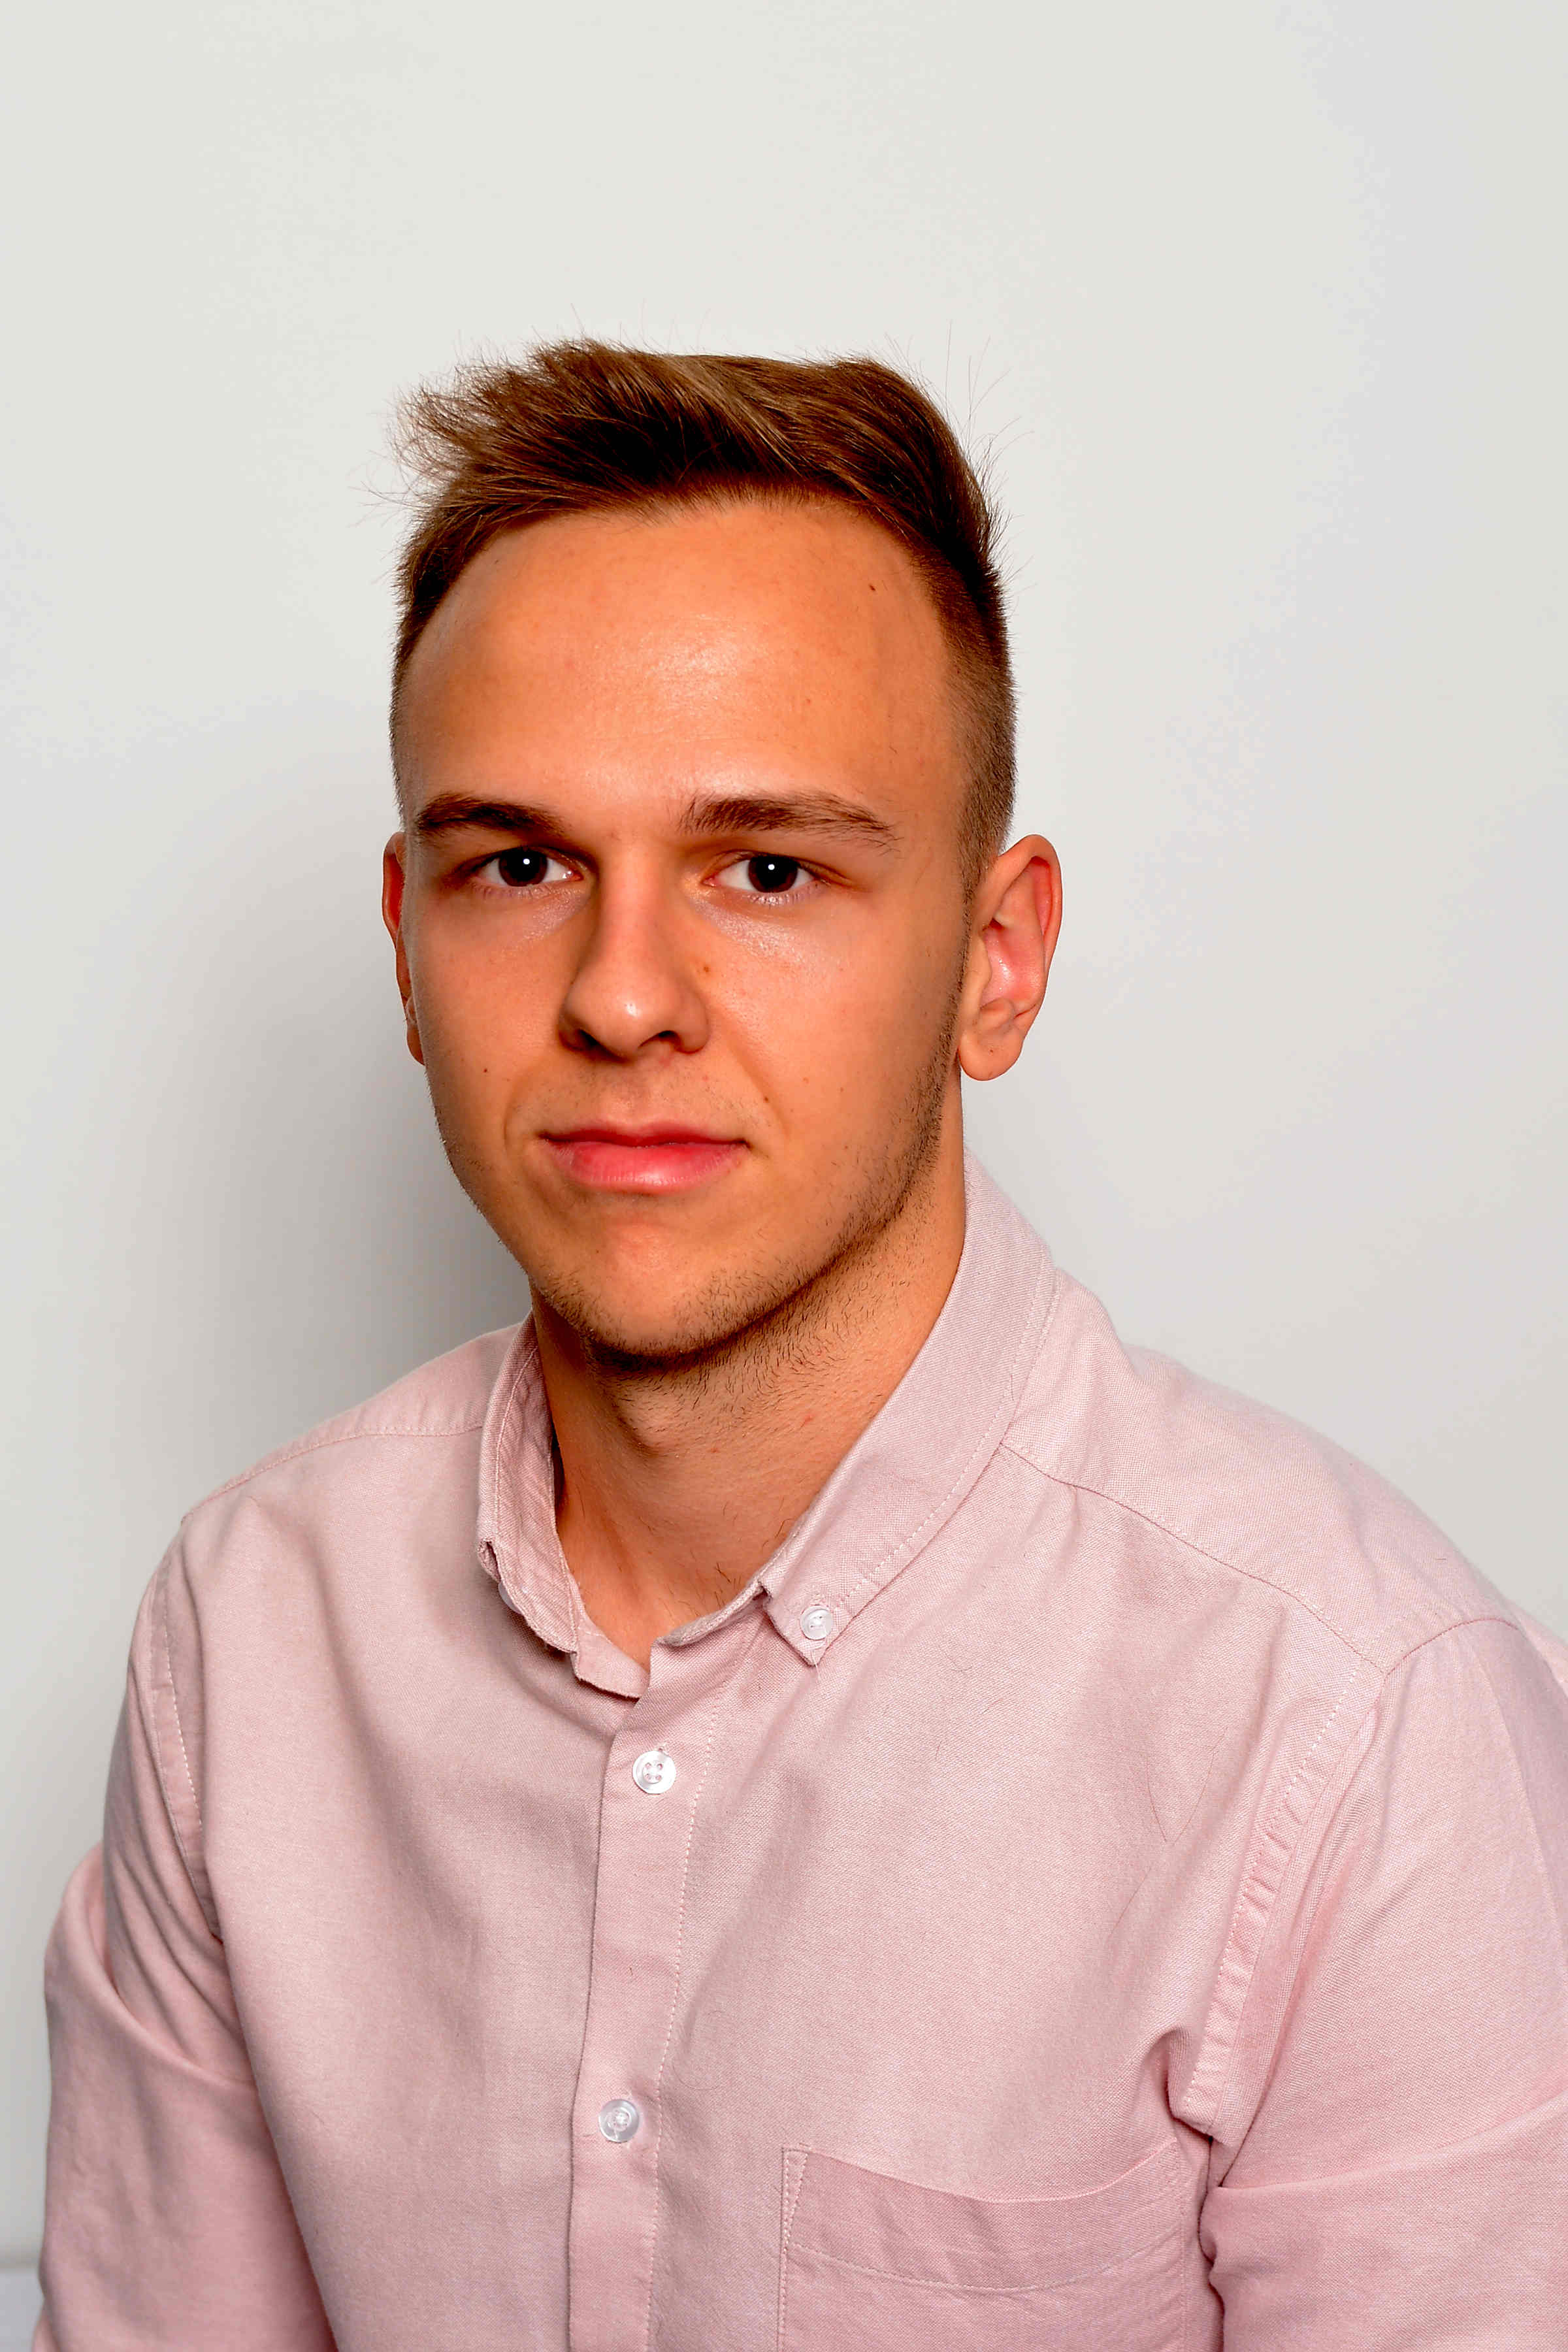
\includegraphics[width=.7\textwidth]{./assets/portrait.jpg}};
\end{tikzpicture}

\vspace{9em}

%%%%%%%%
% EDUCATION %
%%%%%%%%

\heading{Education}

\timelinetable{
	Oct 2017 -- present & \educationentry{Bachelor's: Software Engineering and IT (GPA: 9.84/10)}
	{Faculty of Technical Sciences}
	{University of Novi Sad, Serbia}
	{\newline Courses and more info at: \href{http://bit.ly/2RaGBi0}{\tt http://bit.ly/2RaGBi0}}
}

%%%%%%%%%%%%
% WORK EXPERIENCE %
%%%%%%%%%%%%

\heading{Work Experience}

\timelinetable{
	Oct '20 -- Mar '21 &	\educationentry{Intern}{SAP}{Walldorf, Germany}{\newline
Member of \textit{TI \& HA - Data Management and Platform}. Mainly worked around \textbf{improving caching architecture
for user authorization throughout the cloud system}. Wrote code in Go, infrastructure in Docker and K8s. Also did some
tooling support.
}

\\
    Oct '19 -- Jan '20 & 	\educationentry{Student Demonstrator}{Faculty of Technical Sciences}{Novi Sad, Serbia}{\newline 
Courses: \renewcommand{\labelitemi}{$\textendash$} % Dash instead of dots
 \begin{compactitem}
	\item {\bfseries Object Oriented Programming 2} - Advanced Concepts of OOP using C++ 
	\item {\bfseries System Programming 1} - Assembler, Compiler, Loader and Linker; Grammars
\end{compactitem}
}
}

%%%%%%%%
% PROJECTS %
%%%%%%%%

\heading{Projects}

\timelinetableprojects{
present & \projectentry{\begin{tabular}{@{}l c c c c c c c c c c}\textit{Research} & \textendash & Go & \textendash & Concurrency \end{tabular}}{Go Pipelines (Bachelor Thesis)}{\href{https://github.com/ele7ija/go-pipelines}{\tt github.com/ele7ija/go-pipelines}}
{Looking at applications of \textit{Pipe-and-Filter} pattern in Go. Applying serial and parallel filters on a real-world example. Performance analysis.} \vspace{0.75em} \\ 
2020 & \projectentry{\begin{tabular}{@{}l c c c c c c c c c c}\textit{Commercial} & \textendash & Python (Django) & \textendash & Amazon S3 & \textendash & PostgreSQL & \textendash & Heroku \end{tabular}}{Civil Engineering Company's website}{available at: \href{https://doostabilnost.rs}{\tt doostabilnost.rs}}
{A website for a local company I developed from zero and deployed. For BLOB storage I used S3 and PostgreSQL for relational data.} \vspace{0.75em} \\ 
2021 & \projectentry{\begin{tabular}{@{}l c c c c c c c c c c}\textit{Uni project} & \textendash & Fullstack & \textendash & Document-based  & \textendash & XML & \textendash & RDF & \textendash & Docker \end{tabular}}{Information System for Comissioner For Information of Public Importance's office}{\href{https://github.com/ele7ija/xml-web-services}{\tt github.com/ele7ija/xml-web-services}}
{An extensive Information System that manages all sorts of documents in the process of requesting the information of public importance. Strong use of XML and RDF stores.} \vspace{0.75em} \\
2021 & \projectentry{\begin{tabular}{@{}l c c c c c c c c c c}\textit{Uni project} & \textendash & Fullstack & \textendash & Security  & \textendash & x.509 Certificates & \textendash & Keycloak & \textendash & Docker \end{tabular}}{Hospital Security System}{\href{https://github.com/djuricmilan/BSEP_T13}{\tt github.com/djuricmilan/BSEP\_T13}}
{A general Information System that encompases Hospitals and various Devices in hospitals with a goal of securing their inter-communication. A custom CA infrastructure was involved.}}
% ARCHIVE
% 2019 & \projectentry{\begin{tabular}{@{}l c c c c c c c c}\textit{Application} & \textendash & Java & \textendash & Swing & \textendash & PowerDesigner & \textendash & XML\end{tabular}}{Smart Home}{\href{https://gitlab.com/bpoprzen/smart_home}{\tt gitlab.com/bpoprzen/smart\_home}}{Desktop Java application for generating XML files based on user inputs in GUI.}


%%%%%%
% SKILLS %
%%%%%%

%\heading{Skills}
%\begin{compactitem}
%	\item \textit{Web} - Full-stack; interested in MEVN stack; familiar with Django, Java Spark, Vue.js
%	\item \textit{Interests} - Distributed systems, Systems design, AWS deployments, Messaging, Deep RL
%	\item \textit{Software Development tools and practices} - Maven, {\tt git}, eclipse, Postman, PowerDesigner
%	\item \textit{Competitive Programming} - Went to competitions organized by the Information Society of Serbia in High School; went to a few other hackathons and competitions
%	\item \textit{Languages}: Serbian, English (C1), German (A2)
%\end{compactitem}
%\vspace{1em}

%%%%%%
% About me 
%%%%%%%%
\vspace{0.5em}

\heading{About me}

Hi, I am a motivated \textbf{software engineer} who loves to deeply understand a technology so that 
it can be leveraged in the best way possible. 

\vspace{1em}
My current focus is on \textbf{Cloud Technologies} as a whole and my language of choice is \textbf{Go}. 
I've also done numeruous Full-Stack projects mostly in Uni and had one solo commercial project.  

\vspace{1em}
You can find my contact details at the top of the first page.



%%%%%%%%%%%%%%%%%%%
% END OF DOCUMENT %
%%%%%%%%%%%%%%%%%%%

\end{document}


